\chapter{Grundlagen}
\label{cha:grundlagen}

In diesem Kapitel werden verschiedene in der Masterarbeit verwendete Begriffe, Technologien und Funktionsweisen näher erläutert. Dabei werden die grundlegenden Inhalte geklärt, welche für das Verständnis der Masterarbeit notwendig sind.

\section{Conversational User Interface}
\label{sec:conversational-user-interface}

\aclp{CUI} erlauben es Menschen, durch natürliche Sprache mit Maschinen zu kommunizieren. Diese Idee stellt einen Paradigmenwechsel gegenüber der heute meist verbreitetsten Mensch-Maschine-Interaktion, englisch auch \ac{HCI}, in Form von \aclp{GUI} dar \cite{techlabs_what_2017}. Die Kommunikation erfolgt dabei meist verbal oder textuell. Prinzipiell gehören aber auch Steuerungen via Gestik oder Mimik zu den \acp{CUI}. Im Rahmen dieser Arbeit liegt der Fokus aufgrund der Entwicklung eines Chatbots allerdings auf textbasierten \aclp{CUI}.

\subsection{Entwicklung}
\label{subsec:cui-entwicklung}
\aclp{CUI} haben eine lange Geschichte hinter sich \mbox{\cite[S. 51]{mctear_conversational_2016}}. Bereits in den 1960er Jahren wurden textbasierte Dialogsysteme zum Beantworten von Fragen entwickelt. In den späten 1980er Jahren folgten die ersten sprachbasierten Systeme. In \cite[S. 167]{heinemann_neuausrichtung_2018} wird \textit{Karl Klammer} (oder englisch auch \textit{Clippy}) aus Microsoft Office 1997 sogar als erster Chatbot bezeichnet. Dieser ist mit der Intelligenz von heute bereits verfügbaren Chatbots natürlich nicht zu vergleichen. Grundsätzlich verfolgt er jedoch den verwandten Ansatz, den Nutzer auf natürliche Art und Weise bei der Bedienung des Programms zu unterstützen.

Aufgrund der in den früheren Jahren unausgereiften Technik im Bereich der \acp{CUI} wurde sich zunächst anderen \acp{UI} bedient. So stand zu Beginn der Computergeschichte ausschließlich eine Tastatur zur Eingabe von Befehlen in \acp{CLI}, wie zum Beispiel \acsu{MS-DOS}, zur Verfügung. Im Laufe der Jahre entwickelten sich daraus die ersten \aclp{GUI}, welche zusätzlich mit einer Maus bedient werden konnten. Spätestens mit dem Verkaufsstart der ersten Generation des \textit{iPhones} im Juni 2007 \cite{molla_how_2017} hat der revolutionäre Touchscreen einen festen Platz im Portfolio der \aclp{GUI} eingenommen. In den vergangen Jahren haben die \acp{CUI} derartige Fortschritte gemacht, dass sie sich nahtlos in die Entwicklung der User Interfaces einreihen. In Abbildung \ref{fig:evolution-ui} ist die Entwicklung der \aclp{UI} nochmals in einem Bild festgehalten. Die Bildüberschrift \textit{The Evolution of \ac{UI}} bezieht sich in diesem Zusammenhang nicht auf die Verbesserung, sondern lediglich auf die chronologische Entwicklung der \aclp{UI}. Dabei steht die sprachbasierte Lösung ganz rechts stellvertretend für alle \aclp{CUI}.
\newline

\begin{figure}[htb]
    \centering
    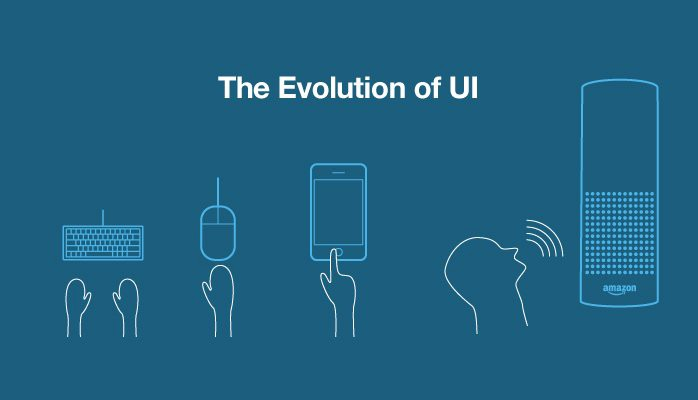
\includegraphics[width=0.9\textwidth]{bilder/evolution-ui.jpg}
    \caption{Chronologische Entwicklung von \aclp{UI} \cite{techlabs_what_2017}}
    \label{fig:evolution-ui}
\end{figure}

\subsection{Grundbegriffe}
\label{subsec:cui-grundbegriffe}

Im Folgenden werden einige Grundbegriffe, die immer wieder in Kombination mit \acp{CUI} vorkommen, erläutert.

Für den Begriff \textbf{\ac{KI}} oder \textbf{\ac{AI}} existiert eine Vielzahl von Definitionen und Interpretationen. Grundsätzlich zielt er darauf ab, einer Maschine intelligentes Verhalten anzueignen. Nach einer der ersten Definitionen für \ac{KI} von Alan M. Turing ist ein System dann intelligent, wenn es in seinen Antworten und Reaktionen nicht von einem Menschen zu unterscheiden ist \cite[S. 237]{nahrstedt_algorithmen_2012}. Der Begriff wird im Zusammenhang mit vielen anderen Forschungsbereichen verwendet, wie zum Beispiel intelligentem menschlichen Verhalten oder Entscheidungsfindung. Bezogen auf \aclp{CUI} bedeutet \acl{KI}, die Bedeutung eines Satzes herauszufinden und zuzuordnen. Dabei darf es keine Rolle spielen, wie der Nutzer seine Intention ausdrückt. \cite[S. 52]{nishith_pathak_artificial_2017}

\textbf{\ac{NLP}} beschreibt Techniken und Methoden zur maschinellen Verarbeitung natürlicher Sprache. Das Ziel ist es dabei, mit der Entwicklung neuartiger Applikationen die Interaktion zwischen Mensch und Maschine auf Basis von natürlicher Sprache zu verbessern \cite[S. 1]{deng_deep_2018}. Häufig ist in diesem Zusammenhang auch von \textbf{\ac{NLU}} die Rede, was einen Teilbereich von \ac{NLP} darstellt. Bei \ac{NLU} geht es dabei explizit darum, einen eingegebenen Text zu interpretieren und Informationen oder Intentionen daraus zu \mbox{gewinnen \cite[S. 15]{ovchinnikova_integration_2012}}.

\textbf{\ac{ML}} bezeichnet ein fundamentales Konzept zum Realisieren von \ac{KI}. Dadurch kann ein System auf Basis von Datenbeständen und Algorithmen  dazulernen, Vorhersagen treffen, Muster erkennen oder Lösungen entwickeln \cite[S. 9]{nishith_pathak_artificial_2017}. \ac{ML} ermöglicht einem System somit Entscheidungen zu treffen, ohne dass diese zuvor explizit programmiert oder vordefiniert werden \cite[S. 187]{mitrevski_developing_2018}. 

\textbf{\ac{DL}} ist eine Technik aus dem Bereich \acl{ML}. In diesem Bereich sind so genannte \acp{ANN}, quasi Modelle nach dem Vorbild von biologischen neuronalen Netzen, weit verbreitet. Mit Hilfe von \ac{DL} und der heute zur Verfügung stehenden Rechenleistung ist es nun möglich, diese sehr rechenintensiven Netzwerke schneller und zuverlässiger abzuarbeiten als herkömmliche Methoden des \aclp{ML}. Für ein möglichst intelligent und zuverlässig arbeitendes System sind dazu riesige Datenmengen, in diesem Zusammenhang oft als \textbf{Big Data} bezeichnet, nötig. \cite[S. 9]{nishith_pathak_artificial_2017}\cite[S. 9-10]{vieira_introduction_2018}

Der Begriff \textbf{\ac{DM}} bezeichnet das Systemverhalten in Abhängigkeit von Nutzeranfragen. Dabei können neben der Intention des Nutzers auch weitere Informationsquellen, wie der Gesprächsverlauf oder Ergebnisse aus Datenbankabfragen relevant sein. Die Komplexität des \ac{DM} kann dabei je nach Umfang und Eigenschaften des Systems variieren. \cite[S. 209-210]{mctear_conversational_2016}

Zwei der wichtigsten Begriffe im Bereich \ac{CUI} sind  \textbf{Intents} und \textbf{Entities}. Der \textit{Intent} gibt an, welches Vorhaben der Nutzer umsetzen will. Dazu wird die textuelle Nutzeranfrage mit Hilfe von \ac{NLU} verarbeitet und daraus der Intent extrahiert. Ist die Intention erkannt, kann eine entsprechende Aktion ausgeführt werden. Die Begriffe Intent, Intention und Vorhaben können im Verlauf dieser Arbeit als gleichwertig betrachtet werden. \textit{Entities} sind wichtige Parameter oder Schlüsselwörter in einer Nutzeranfrage. Entitäten geben wichtige Zusatzinformationen zu einem Intent an und können helfen, diesen überhaupt erst zu identifizieren. Dabei gibt es sowohl Systementitäten (z.B. Wochentag) als auch userspezifische Entitäten (z.B. Flugzeugtyp). \cite[S. 27, 44-45]{khan_build_2018}\cite[S. 12-13]{mitrevski_developing_2018} \\
Dies soll anhand eines Beispiels verdeutlicht werden. Die verwendeten Bezeichnungen für Intents, Entitäten und Parameter sind fiktiv und dienen lediglich dem besseren Verständnis. 

\begin{center}
Nutzer: \textit{„Kannst du mir einen Flug von \colorbox{SkyBlue}{Nürnberg} nach \colorbox{YellowGreen}{Berlin} buchen?“} \\
\colorbox{Peach}{[Intent erkannt: BucheFlugIntent]} \\
Chatbot: \textit{„Wann möchtest du fliegen?“}\\
Nutzer: \textit{„Am \colorbox{Rhodamine}{Freitag}“} \\
Chatbot: \textit{„Ich habe folgende Flüge gefunden.“} \\
\end{center}

Aus der ersten Frage des Nutzers kann der Intent \textbf{\textcolor{Peach}{\textit{BucheFlugIntent}}} sowie die beiden Entitäten \textbf{\textcolor{SkyBlue}{\textit{Abflughafen}}} und \textbf{\textcolor{YellowGreen}{\textit{Zielflughafen}}} ermittelt werden. Es fehlt allerdings noch die Auskunft nach dem Tag des Abflugs. Das System arbeitet dabei über eine Rückfrage und erwartet als Antwort einen Wert der Systementität \textit{Wochentag}. Gibt der Nutzer eine entsprechende Antwort (z.B. \textbf{\textcolor{Rhodamine}{\textit{Freitag}}}), hat das System alle notwendigen Daten erhalten und kann über ein entsprechendes \acl{DM} eine Antwort generieren.

\subsection{Chatbot}
\label{subsec:cui-chatbot}

Der Begriff Chatbot oder auch Chatterbot setzt sich aus den beiden Begriffen \textit{chat} \mbox{(= Gespräch)} und \textit{bot} (= Kurzform für Roboter) zusammen. In der Informatik wird ein Bot als weitgehend selbstständig laufendes Programm bezeichnet. Ein Chatbot ist somit eine Softwareanwendung zur Realisierung einer Unterhaltung zwischen Mensch und Maschine \cite[S. 232]{smolinski_innovationen_2017}. Die meisten Chatbots sind derzeit textbasiert, einige bieten allerdings auch die Möglichkeit der sprachlichen Ein- und Ausgabe. Das Ziel ist es dabei, dem Chatbot intelligentes Verhalten anzueignen und ihn dadurch für unterschiedlichste Aufgaben verwenden zu können. Um dies zu ermöglichen, werden die in \ref{subsec:cui-grundbegriffe} beschriebenen Techniken angewendet.

Einer der größten Vorteile von Chatbots im Vergleich zu herkömmlichen mobilen Applikationen ist, dass der Nutzer dem System sein Vorhaben auf natürliche Art und Weise mitteilt. Nach einer Statistik aus \cite{mcgrath_when_2018} haben immer noch 70\,\% der Menschen in reichen Ländern mangelnde oder gar keine Computerkenntnisse. \aclp{CUI} und damit auch Chatbots umgehen diese Probleme, da alle Menschen den natürlichen Gesprächsdialog kennen und verstehen. Aus Entwicklersicht ist die Verarbeitung von natürlicher Sprache jedoch schwieriger zu handhaben als beispielsweise ein \acl{UI} mit verschiedenen Buttons. Zwar funktioniert das mit modernsten \ac{NLP}-Plattformen wie \textit{Dialogflow} bereits erstaunlich gut, allerdings gibt es bei komplizierteren oder ungewöhnlicheren Formulierungen noch Probleme. Ein anderer Ansatz ist es dabei, das \acl{CUI} mit Visualisierungen zu erweitern. So kann beispielsweise eine Rückfrage seitens des Chatbots schnell und einfach durch eine Auswahl an Popup-Buttons beantwortet werden. Die Textbox am unteren Ende wird dabei zu jeder Zeit angezeigt und bietet dem Nutzer die Möglichkeit zur textbasierten Kommunikation. Mittels einer \textit{Web View} können dabei ganze \acs{HTML}-Seiten geladen und angezeigt werden. Verwendet werden sie für Aufgaben, die für ein chatbasiertes \acl{UI} nur schwer oder gar zu kompliziert umzusetzen \mbox{sind. \cite[S. 7-10]{khan_build_2018}}

Hinsichtlich der Architektur gibt es eine Reihe verschiedener Technologien, Frameworks und Plattformen um einen Chatbot zu realisieren. Im Folgenden soll daher eine Möglichkeit vorgestellt werden, die sich im Rahmen einer Recherche als plausibel und auch für die weitere Arbeit nutzbar herausgestellt hat. Das Schaubild dazu zeigt Abbildung \ref{fig:aufbau-chatbot}.

Ein \textit{User} schreibt zu Beginn der Konversation eine Nachricht über eine \textit{Messaging Platform} an das \textit{\acl{NLP}} Tool. Es gibt einige Nachrichtenplattformen, in denen Chatbots entwickelt und integriert werden können. Vorreiter in diesem Gebiet war vor allem der chinesische Messenger \textit{WeChat}, ehe in den letzten Jahren weitere Nachrichtenplattformen wie beispielsweise der \textit{Facebook Messenger} oder \textit{Slack} nachzogen \cite{rocketbots.io_china_2017}. Nach \cite{riya_study_2018} sind im Bereich \acl{NLP} derzeit die Plattformen \textit{Dialogflow, Wit.ai, Amazon lex, Luis} und \textit{IBM Watson} marktführend. Diese Plattformen kümmern sich um das \acl{NLU} und ordnen den Anfragen die Intents und Entities zu. 

Die \textit{Bot-Logic} interpretiert die Nachricht und leitet sie an das Backend, in der Abbildung \ref{fig:aufbau-chatbot} als \textit{Information Sources} dargestellt, weiter. Durch immer mehr Nutzeranfragen wird der Chatbot trainiert und kann sich dadurch stetig verbessern. Dahinter steckt das in \ref{subsec:cui-grundbegriffe} erklärte Prinzip des \textit{\acl{ML}}. Im Backend findet dann üblicherweise das \acl{DM} statt. Hier werden die Informationen verarbeitet und Entscheidungen in Form von \textit{Actions} getroffen. 

Zudem können gegebenenfalls weitere Informationsquellen, beispielsweise aus \textit{Datenbanken}, angebunden werden. Außerdem ist es möglich \textit{\acp{API}} wie zum Beispiel die \textit{Google Calendar API} zum Verwalten von Terminen in das Backend einzubinden. Gibt es Probleme mit der Dialogführung oder kommt der Chatbot an seine Grenzen, kann die Nachricht an einen echten Menschen, in der Darstellung als \textit{Human Intervention} bezeichnet, weitergeleitet werden. \cite{fourault_ultimate_2017}
\newline

\begin{figure}[htb]
    \centering
    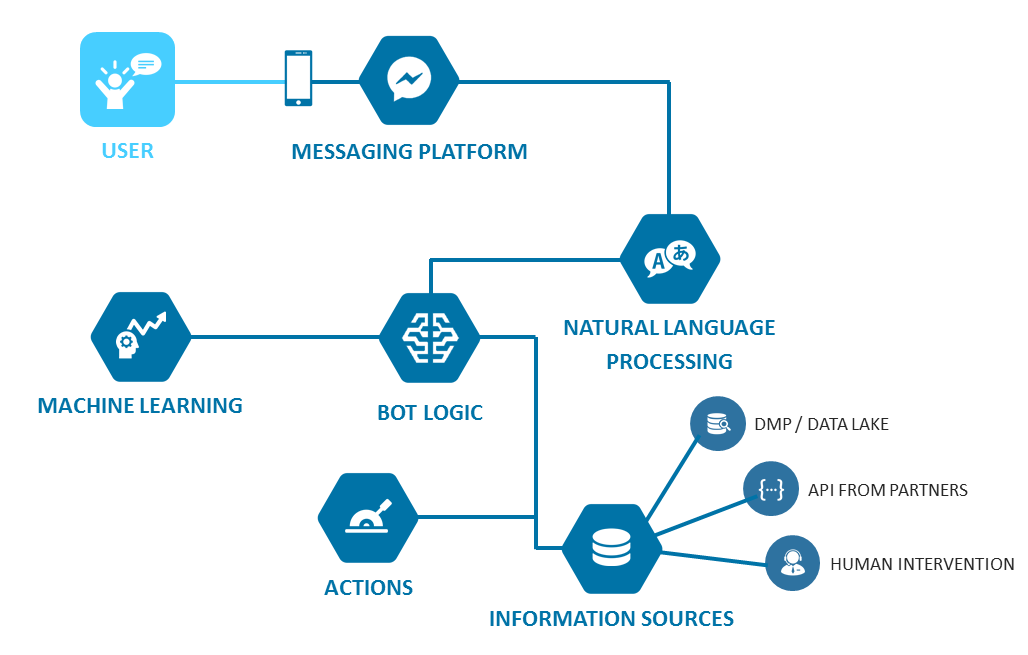
\includegraphics[width=1\textwidth]{bilder/aufbau-chatbot_v2.png}
    \caption{Aufbau eines Chatbots \cite{fourault_ultimate_2017}}
    \label{fig:aufbau-chatbot}
\end{figure}

\newpage
\section{Android Applikation}
\label{sec:basics-android-applikation}

Das Smartphone-Betriebssystem \textit{Android} hat derzeit in Deutschland einen Marktanteil von etwa 83\,\%\footnote{Stand: September 2018} \cite{statistica.com_marktanteile_2018}. Der Standard für die Entwicklung von Android Applikationen ist \textit{Java}, allerdings wird seit einiger Zeit auch \textit{Kotlin} vollständig unterstützt. Kotlin ist eine statisch typisierte Programmiersprache, die auf \ac{JVM} basiert. Einer der größten Vorteile ist dabei, dass Java und Kotlin gemeinsam innerhalb eines Projekts genutzt und sogar automatisch in die jeweils andere Sprache übersetzt werden können. Entwickelt wurde Kotlin von der Firma  \textit{JetBrains}, die auch die Entwicklungsumgebung \textit{Android Studio} zur Verfügung stellt. \cite[S. 272]{prasad_reddy_beginning_2017}

\subsection{Manifest}
\label{subsec:basics-android-manifest}

Zu Beginn jeder Android Applikation steht das \textit{Manifest}, repräsentiert durch die Datei \textit{AndroidManifest.xml}. Es nutzt \ac{XML} und dient als zentraler Punkt zur Deklaration von wichtigen Informationen über die App und ihre Komponenten. Hier werden unter anderem Aktivitäten, Services und Berechtigungen eingetragen \cite[S. 41]{allen_beginning_2015}. Im Folgenden ist eine beispielhafte Manifest Datei dargestellt, welche einen grundlegenden Eindruck vom Aufbau vermitteln soll.
\newline

\begin{lstlisting}[caption={Beispielhafte AndroidManifest.xml Datei}, captionpos=b, label={lst:manifest-xml}, language=XML]
<?xml version="1.0" encoding="utf-8"?>
<manifest xmlns:android="http://schemas.android.com/apk/res/android"
    package="com.example.michaelwagner.beispiel">
    
    <uses-permission android:name="android.permission.INTERNET"/>
    
    <application
        android:allowBackup="true"
        android:icon="@mipmap/ic_launcher"
        android:label="@string/app_name"
        android:roundIcon="@mipmap/ic_launcher_round"
        android:supportsRtl="true"
        android:theme="@style/AppTheme">
        <activity android:name=".Activities.MainActivity">
            <intent-filter>
                <action android:name="android.intent.action.MAIN" />
                <category android:name="android.intent.category.LAUNCHER" />
            </intent-filter>
        </activity>
        <activity android:name=".Activities.SecondActivity"></activity>
    </application>
</manifest>
\end{lstlisting}

Der Name hinter dem Tag \textit{package} dient der Identifikation der App auf dem Smartphone oder auch im \textit{Google Play Store}. Durch die Angabe von \textit{uses-permission} können diverse Berechtigungen, wie hier etwa \textit{INTERNET} zur Herstellung von Internetverbindungen, erteilt werden. Einige häufig verwendete Permissions sind \textit{CAMERA} für Kamerazugriff, \textit{ACCESS\_FINE\_LOCATION} für den genauen Standort und \mbox{\textit{RECORD\_AUDIO}} zur Sprachaufnahme via Mikrofon. Das Element \textit{application} definiert das Anfangsverhalten der App. Die Attribute für \textit{icon}, \textit{label} oder \textit{theme} definieren Basisinformationen wie das Icon oder den Namen für die App. Außerdem muss jede \textit{activity} dort eingetragen sein. Dabei muss auch eine \textit{Launcher Activity} deklariert werden, die der Nutzer als Erstes beim Start der App sieht.. \cite[S. 42-43]{allen_beginning_2015}\cite{android_developers_app_2018}

\subsection{Layout}
\label{subsec:basics-android-layout}

Wie schon beim Manifest wird auch für das Layout einer Android App die erweiterbare Auszeichnungssprache \ac{XML} genutzt. Das Layout definiert den Aufbau des \aclp{UI}. Unterschieden werden dabei \textit{View}- und \textit{ViewGroup}-Objekte. Eine ViewGroup ist eine Art unsichtbarer Container, der die Struktur für weitere Elemente vorgibt. Jede Layout-Datei besitzt dabei genau eine übergeordnete ViewGroup, die für das gesamte \ac{UI} gilt. Nach \cite[S. 79-80]{allen_beginning_2015} sind die am häufigsten verwendeten Layout-\mbox{Container}:
\begin{itemize}
\item\textbf{RelativeLayout} - Verschiedene Regeln zur relativen Anordnung der Elemente unter-, über- oder nebeneinander 
\item\textbf{LinearLayout} - Alle Elemente werden in einer Richtung, horizontal oder vertikal, angeordnet
\item\textbf{ConstraintLayout} - Keine verschachtelten ViewGroups, alle Elemente werden relativ angeordnet, über so genannte Constraints (Regeln)
\end{itemize}

Eine View ist die Basisklasse eines \textit{Widgets}, wie \textit{Button} oder \textit{TextView}. Widgets werden genutzt, um ein interaktives \acl{UI} zu erstellen \cite[S. 137]{jackson_learn_2013}. Die Views und ViewGroups unterstützen verschiedene Attribute. Dabei gibt es sowohl Attribute für alle Elemente als auch spezifische Attribute, die nur bestimmte Elemente implementieren können. Generell sollten bei der Angabe von Höhe, Breite oder Schriftgröße konstante Werte vermieden werden. Besser ist die Angabe von relativen Maßen wie \textit{\ac{dp}}, \textit{wrap\_content} oder \textit{match\_parent}, weil dadurch sichergestellt wird, dass die App auch auf unterschiedlichen Bildschirmgrößen korrekt dargestellt wird. Tabelle \ref{tab:attributes-layout-elements} zeigt eine kleine Auswahl an Attributen inklusive Beispielwert und Bedeutung. \cite{android_developers_layouts_2018}
\newline
\def\arraystretch{1.5}
\begin{table}[ht!]
    \centering
    \begin{tabular}{| C{3.5cm} | C{2.5cm} | C{7cm} | } 
    \hline \textbf{Attribut} & \textbf{Beispielwert} & \textbf{Bedeutung} \\ [0.5ex] 
    \hline android:id & @+id/my\_button & Eindeutiger Identifier des Elements \\
    \hline android:layout\_width & wrap\_content  & Breite des Elements an Inhalt anpassen \\
    \hline android:layout\_height & match\_parent & Höhe des Elements wie übergeordnetes Element  \\
    \hline android:text & Das ist ein Text & Textinhalt des Elements \\
    \hline android:textSize & 12dp & Schriftgröße des Elements \\
    \hline android:background & \#f9aa20 & Hintergrundfarbe des Elements \\
    \hline
    \end{tabular}
    \caption{Attribute von Layout-Elementen}
    \label{tab:attributes-layout-elements}
\end{table}

\subsection{Activity}
\label{subsec:basics-android-activity}

Eine Aktivität (engl. \textit{Activity}) repräsentiert einen Bildschirm, mit dem der Nutzer interagieren kann. Die Aktivität selbst stellt dabei in der Regel keine Benutzeroberfläche bereit, sondern ist mit einem entsprechen \ac{XML}-Layout verknüpft. Ein äußerst wichtiges Prinzip im Zusammenhang mit Aktivitäten ist der Lebenszyklus. Dabei werden Aktivitäten via \textit{Callback}-Methoden über Zustandsänderungen informiert. Jede dieser Methoden kann überschrieben werden. \cite[S. 187-188]{gerber_learn_2015}\cite{programmieren_lernen_programmier_2018} 

\clearpage
Die verschiedenen Zustände und dazugehörigen Methoden werden im Folgenden anhand von Abbildung \ref{fig:android-lebenszyklus-acitvity} ausführlich erläutert. 

\begin{itemize}
\item\textbf{onCreate()}: Wird beim erstmaligen Erzeugen der Aktivität aufgerufen. Hier sollten Initialisierungen vorgenommen, Views erzeugt oder Daten geladen werden. Anschließend wird \textit{onStart()} aufgerufen.

\item\textbf{onRestart()}: Die Aktivität muss zuvor gestoppt worden sein. Der Aufruf erfolgt, wenn User zu der Activity zurück navigiert. Der Methode folgt immer \textit{onStart()}.

\item\textbf{onStart()}: Wird aufgerufen, kurz bevor die Aktiviät auf dem Bildschirm sichtbar wird. Anschließend wird \textit{onResume()} aufgerufen. 

\item\textbf{onResume()}: Diese Methode wird ausgeführt, wenn die Aktivität bereit für Benutzereingaben ist. Nach Beendigung dieser Methode wird die Aktivität ausgeführt.

\item\textbf{onPause()}: Wird kurz vor dem Start einer anderen Aktivität aufgerufen. Geänderte Daten oder Zustände sollten an dieser Stelle gespeichert werden. Anschließend wird \textit{onResume()} aufgerufen, wenn die Activity wieder in den Vordergrund rückt oder \textit{onStop()}, wenn sie verdeckt wird. 

\item\textbf{onStop()}: Wird aufgerufen, wenn die Aktivität nicht mehr sichtbar ist. Nach dieser Methode kann das Android-System den App-Prozess aufgrund von Speicherplatzmangel direkt beenden. Anschließend folgt die \textit{onRestart()} Methode, wenn die Activity wieder fortgesetzt wird oder die \textit{onDestroy()} Methode, wenn die Activity endgültig zerstört wird.

\item\textbf{onDestroy()}: Aufruf kurz vor dem Zerstören der Aktivität. Erfolgen kann dies planmäßig innerhalb der Applikation oder durch das Android-System. Nachdem dies der letzte Aufruf ist, folgt keine weitere Methode.

\end{itemize}

\begin{figure}[htb]
    \centering
    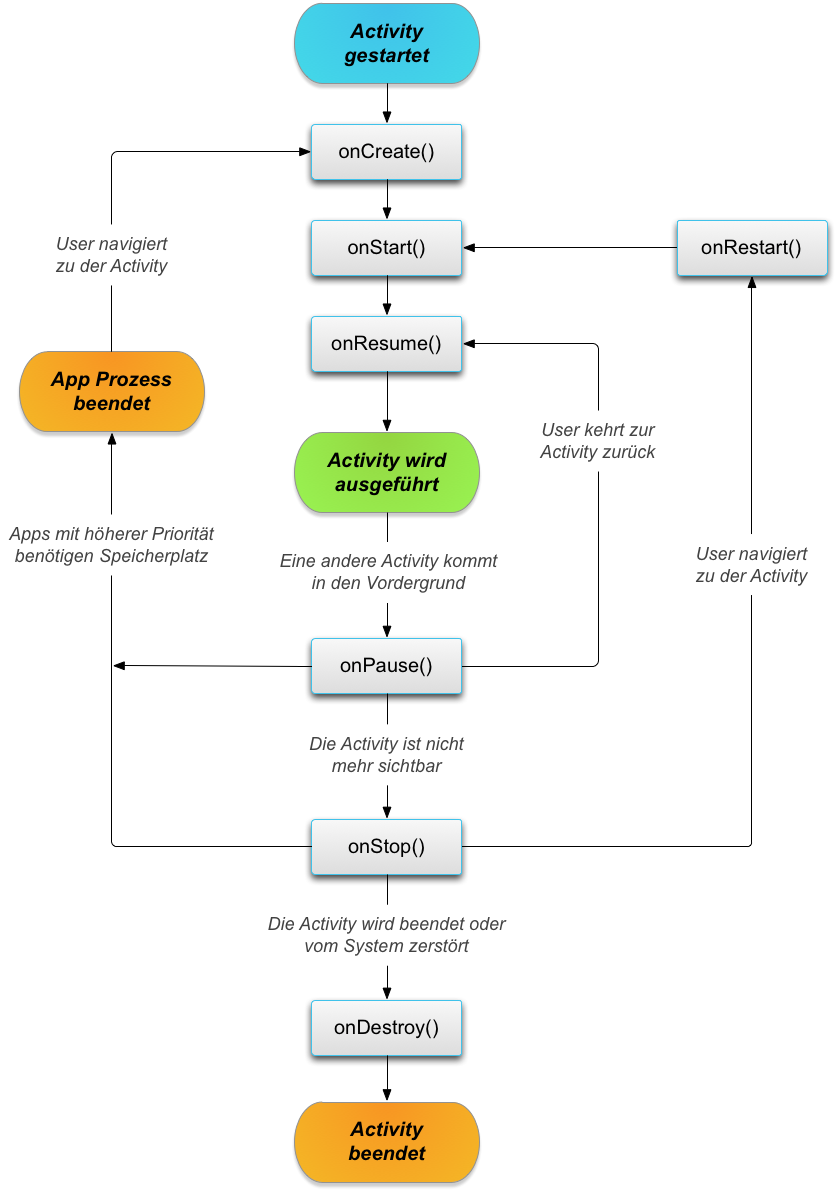
\includegraphics[width=1\textwidth]{bilder/android_activity_lifecycle.png}
    \caption{Lebenszyklus einer Aktivität \cite{programmieren_lernen_programmier_2018}}
    \label{fig:android-lebenszyklus-acitvity}
\end{figure}

